\documentclass[aspectratio=169,10pt]{beamer}
\usepackage[UTF8]{ctex}\usepackage{booktabs,tabularx,amsmath,graphicx}
\usetheme{Madrid}\definecolor{navy}{HTML}{142B43}\definecolor{teal}{HTML}{168579}
\setbeamercolor{structure}{fg=navy}\setbeamercolor{frametitle}{bg=navy,fg=white}
\setbeamercolor{block title}{bg=teal,fg=white}\setbeamercolor{block body}{bg=teal!6}
\setbeamertemplate{navigation symbols}{}\setbeamertemplate{footline}{\leavevmode\hbox{\begin{beamercolorbox}[wd=.79\paperwidth,ht=2.5ex,dp=1ex,leftskip=1em]{author in head/foot}青序量化研究平台\quad CF2026 Project 1\end{beamercolorbox}\begin{beamercolorbox}[wd=.21\paperwidth,ht=2.5ex,dp=1ex,center]{date in head/foot}\insertframenumber/20\end{beamercolorbox}}}
\setbeamerfont{frametitle}{size=\large}\setbeamersize{text margin left=8mm,text margin right=8mm}
\begin{document}
\begin{frame}{青序量化研究平台}
\begin{block}{}从失败账本到超过指数的历史候选\end{block}
\small\begin{itemize}
\item Computational Finance · Project 1
\item 1,000只股票，12因子，8个V3候选
\item 固定复核：2025-01-02 至 2026-09-18
\end{itemize}
\note{本次展示从平台正确性开始，解释原始失败、用户升级的指数目标，以及最后找到的滚动LightGBM候选。必须同时说明：这个候选经过历史结果筛选，不是独立盲测成功。}
\end{frame}

\begin{frame}{Project 1 的核心是研究闭环}
\begin{block}{}基础80分与扩展20分，落实为可检查的证据\end{block}
\small\begin{itemize}
\item 数据：字段、复权、缺失、下载身份与哈希
\item 研究：因子、IC、分组、含费用回测、固定对照
\item 工程：同一核心供CLI和界面调用，保留测试与运行记录
\item 扩展：历史中性化、风险权重、部分成交、增量审计
\end{itemize}
\note{老师的要求没有规定必须达到某个收益或Sharpe。因此我们把正确性和复现放在第一位。每项要求都能从代码追到输出文件：例如因子分组保留形成时人数，成交文件保留实际金额和费用。扩展选择有验证证据的几项，不靠堆页面数。收益研究是平台能力的演示，同时接受失败结果。}
\end{frame}

\begin{frame}{原始动量的亏损超过费用拖累}
\begin{block}{}零费用独立重跑仍累计亏损75.16\%\end{block}
\centering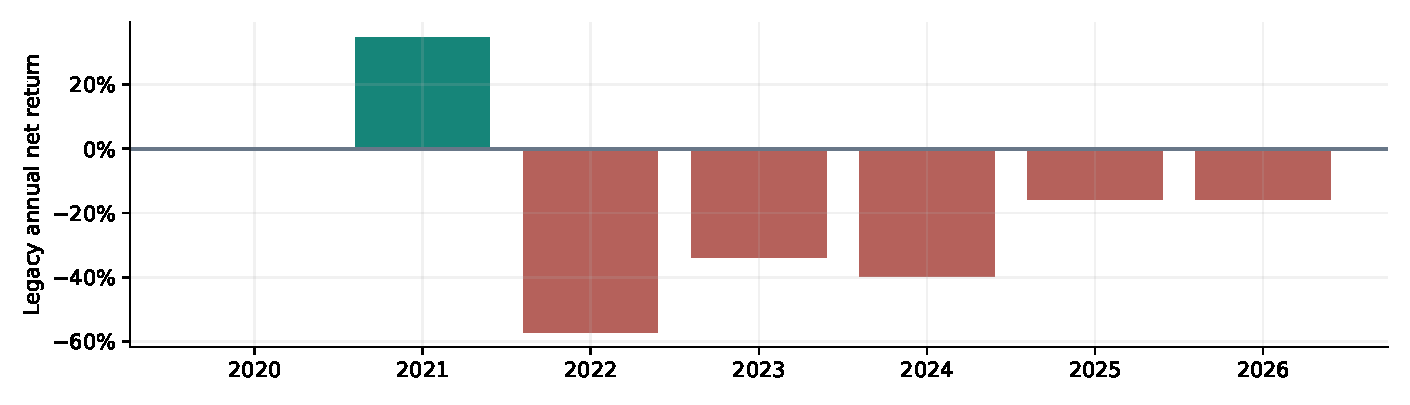
\includegraphics[width=.94\textwidth,height=.51\textheight,keepaspectratio]{figures/legacy.pdf}\par
\scriptsize\begin{itemize}
\item 原始扣费累计：$-$83.57\%，最大回撤89.83\%
\item 加回费用的同路径归因：$-$58.12\%
\item 零费用重跑会改变再投资路径，不能混为一谈
\end{itemize}
\note{原策略用二十日动量，每五个交易日调整前三十只股票。图里可以看到二零二二到二零二四年连续亏损。实际账本扣费亏损百分之八十三点五七，而真正将费用设为零再运行，仍亏损百分之七十五点一六。简单把累计费用加回净值，会得到另一条归因曲线。这个差异说明费用、仓位规模和后续盈亏有路径依赖。我们因此同时改进信号研究与组合构建。}
\end{frame}

\begin{frame}{分数与成交账本解耦}
\begin{block}{}新增模型输出同样的分数接口\end{block}
\small\begin{itemize}
\item 原始快照与质量检查
\item 因子/模型：日期$\times$资产分数
\item 组合模块：目标权重与现金
\item 成交模块：订单、成交、持仓、净值
\end{itemize}
\note{这里是可维护性的关键。模型只回答股票的相对分数，组合层决定多少资金投入，成交层决定订单实际完成多少。将来接入新因子或更复杂模型，不需要再写一套会计逻辑。命令行和界面调用相同函数。每次实验带上数据、参数和源码身份，避免出现界面显示一种口径、报告计算另一种口径。}
\end{frame}

\begin{frame}{1,656,599条日线具有明确来源}
\begin{block}{}固定2019年末股票池，保留后来缺失的成员\end{block}
\begin{center}\small\begin{tabularx}{.96\textwidth}{lX}\toprule
项目 & 结果\\\midrule
资产 / 交易日 & 1,000 / 1,690\\
日线重复键 / 异常剔除 & 0 / 0\\
缺失网格 / 缺限制价 & 33,401 / 48\\
每日估值记录 & 1,656,599\\
\bottomrule\end{tabularx}\end{center}
\small\begin{itemize}
\item 价格区间：2019-10-08 至 2026-09-18
\item 57,389条财务指标，1,432条历史行业区间
\item 原行情3,006个文件、新研究2,073个文件哈希核验
\item 固定池不含后续IPO，也不代表全A股
\end{itemize}
\note{股票池在二零一九年末按当时成交额选取，收益研究从之后开始。我们没有拿今天还上市的股票倒推历史。完整网格有三万三千多条缺失，缺失会影响因子、成交和估值，所以分别处理并计数。补充每日估值、公告和历史行业后，整体本地存储约一点六三GB。最重要的边界是固定池的选择偏差和厂商事后修订，它们不会因为数据量大而自动消失。}
\end{frame}

\begin{frame}{年度更新模型，标签先实现}
\begin{block}{}每年只训练形成日前三年的可见观测\end{block}
\small\begin{itemize}
\item 2023/2024先验证，清除跨形成日标签
\item 2025/2026逐年重训，同一年度固定模型
\item 原V2已看过最终区间，不能恢复盲测资格
\end{itemize}
\note{形成日是每年第一次交易前一个交易日。标签退出日必须严格早于形成日，因此不能把还没实现的20日收益放进训练。每年滚动最近三年训练，随后一年使用新模型。此次最终区间已被V2观察，滚动训练不能改变这个事实。}
\end{frame}

\begin{frame}{12个因子构成可解释的基线}
\begin{block}{}既保留防御与价值，也保留表现不佳的方向\end{block}
\begin{center}\small\begin{tabularx}{.96\textwidth}{lX}\toprule
类别 & 因子\\\midrule
趋势 / 反转 & 跳月动量、5日反转、20日均线趋势\\
风险 / 量价 & 低波动、低振幅、量能变化、流动性、低换手\\
价值 / 分红 & 盈利收益率、账面市值比、股息率\\
质量 & 最新已公告年度ROE\\
\bottomrule\end{tabularx}\end{center}
\small\begin{itemize}
\item 同日横截面统一方向与尺度
\item 至少10个因子有效，其余标准化缺值取中性值0
\item 完整因子卡列出字段、窗口与失败情形
\end{itemize}
\note{这十二个因子并不是十二个独立的信息源。低波动和低振幅就可能高度相关。它们覆盖中期趋势、短期反转、风险、量价、价值和盈利质量。我们提前固定符号，在最终期IC为负时也不直接翻转。参考了Qlib的量价表达，但没有声称完整实现Alpha158。后续需要以独立验证证明新增因子提供额外信息。}
\end{frame}

\begin{frame}{中性化与标准化同时输入}
\begin{block}{}LightGBM使用12个标准化值与12个残差值\end{block}
\small\begin{itemize}
\item 每日1\%/99\%截尾、样本标准差缩放
\item 当日行业与对数市值回归残差
\item 缺财报不补未来值；个别标准化缺值取0
\item 中性化减少暴露，但不保证提高收益
\end{itemize}
\note{保留两套表示让模型区分原始风格和剔除行业市值后的相对位置。全部横截面处理只使用当天数据。基本面严格晚于公告日才可见，但仍披露厂商历史修订。}
\end{frame}

\begin{frame}{候选有明确边界}
\begin{block}{}四种信号 $\times$ 两种组合，共8个候选\end{block}
\small\begin{itemize}
\item 经济主题：价值50\%、质量25\%、低风险25\%
\item Ridge：12个中性化输入，alpha=100
\item LightGBM：24输入、250树、15叶、深度5
\item 融合：树模型50\%、线性25\%、主题25\%
\end{itemize}
\note{候选和容量在本轮开始前写进协议。每种信号配稳定股票仓位和波动预算组合，避免只展示胜出的模型。神经网络仍在V2版本对照中，本轮不要求复杂模型必须胜出。}
\end{frame}

\begin{frame}{仓位目标与指数目标相适应}
\begin{block}{}最高95\%股票敞口；趋势偏弱时预算乘0.75\end{block}
\small\begin{itemize}
\item 20日调仓、50股、20名缓冲
\item 波动目标20\%，单股4\%、行业25\%
\item 其余持现金，禁止杠杆与卖空
\item 实际权重会漂移，回撤目标不是保证
\end{itemize}
\note{上一版平均一半现金更适合防御。新方案提高股票参与度，同时保留波动、行业和单股限制。最新候选最终期平均现金约17.87\%。权重和波动是形成时目标，无法承诺未来回撤上限。}
\end{frame}

\begin{frame}{账本正确与策略达标分开}
\begin{block}{}版本切换后清除旧结果，亏损显示未达标\end{block}
\small\begin{itemize}
\item 新旧策略共用成交与独立核对核心
\item 下一开盘，实际成交收费，限制价/缺价阻断
\item 最新默认V3，V1失败与V2对照仍可选择
\item 固定结果可查看；本机可改参数重跑
\end{itemize}
\note{绿色账本提示曾容易让用户误以为策略合格。现在会分别显示资金核对与收益风险判断。回测页直接提供V1、V2、V3版本，不再只给旧动量入口。}
\end{frame}

\begin{frame}{验证选择没有被事后改写}
\begin{block}{}价值主题稳定仓位排名第一，但随后失败\end{block}
\centering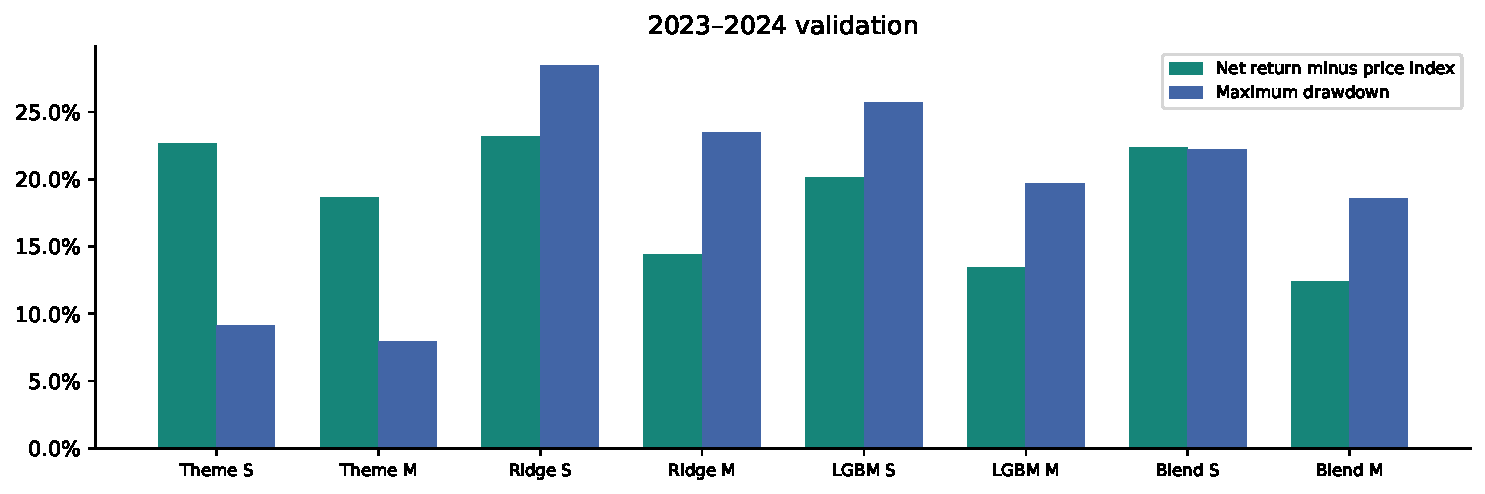
\includegraphics[width=.94\textwidth,height=.51\textheight,keepaspectratio]{figures/validation.pdf}\par
\note{先看2023到2024，规则要求净收益、超额收益为正且回撤不超过25\%，按最差年度超额优先。价值主题稳定仓位被预选。LightGBM稳定仓位回撤25.73\%，没有通过风险门槛。}
\end{frame}

\begin{frame}{历史复核保留全部8个候选}
\begin{block}{}当前候选为滚动LightGBM波动预算版\end{block}
\centering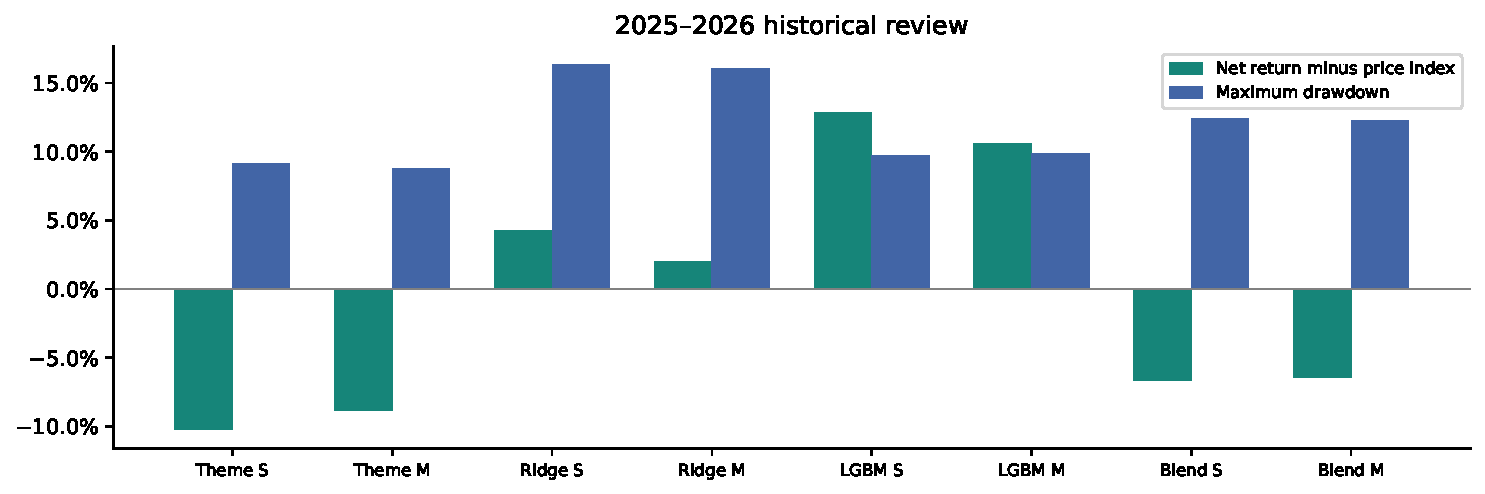
\includegraphics[width=.94\textwidth,height=.51\textheight,keepaspectratio]{figures/test_models.pdf}\par
\note{预选价值主题最后只赚4.30\%，没有超过指数。用户要求继续研究后，我们在通过验证门槛的候选中根据这张历史结果表选择LightGBM波动预算。这是开发后的候选选择，不能说事前选中了赢家。稳定版树模型收益更高，但验证回撤超门槛，未作为默认。}
\end{frame}

\begin{frame}{策略超过价格与全收益指数}
\begin{block}{}净收益25.13\%，最大回撤9.88\%\end{block}
\centering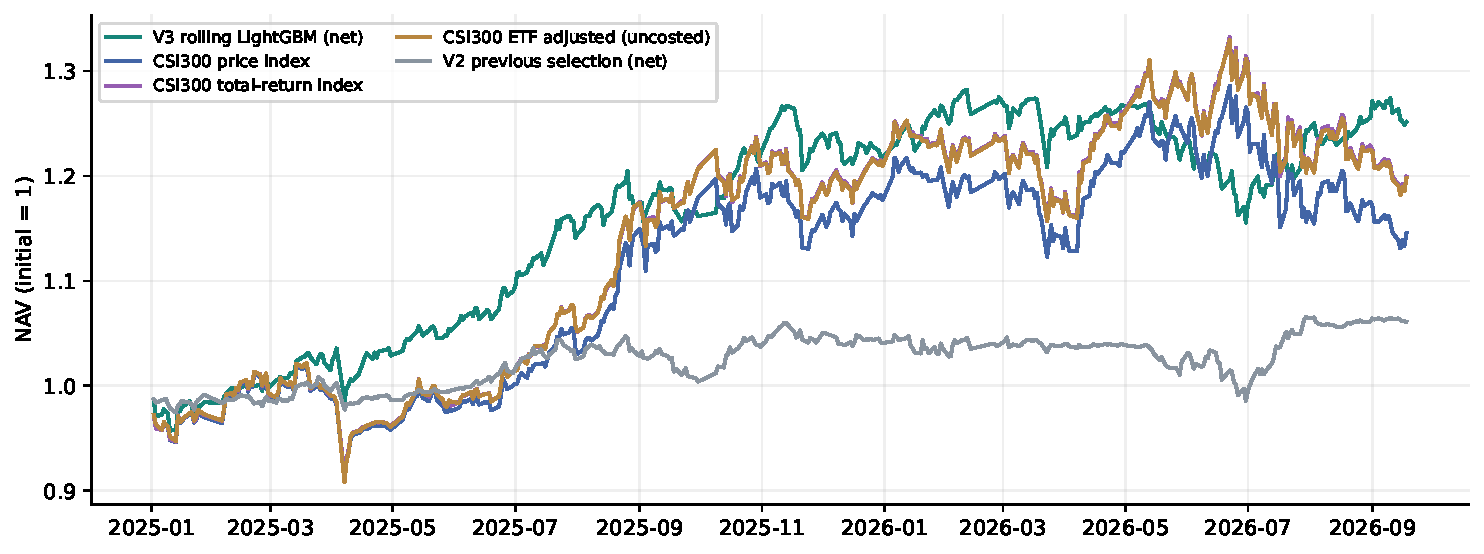
\includegraphics[width=.94\textwidth,height=.51\textheight,keepaspectratio]{figures/nav.pdf}\par
\scriptsize\begin{itemize}
\item 价格指数14.55\%，全收益指数19.94\%
\item 分别超过10.58和5.19个百分点
\end{itemize}
{\tiny 本页展示完整417日净值；PowerPoint版每5个交易日取点。}
\note{该结果覆盖固定417日，费用已扣。全收益指数包含红利再投资，是比价格指数更严格的基准。策略收益25.13\%、年化14.51\%、回撤9.88\%。我们也检查首次开盘基准和ETF代理，结论没有改变。}
\end{frame}

\begin{frame}{加倍费用与延迟信号仍胜出}
\begin{block}{}压力检查不再用于选择更好参数\end{block}
\centering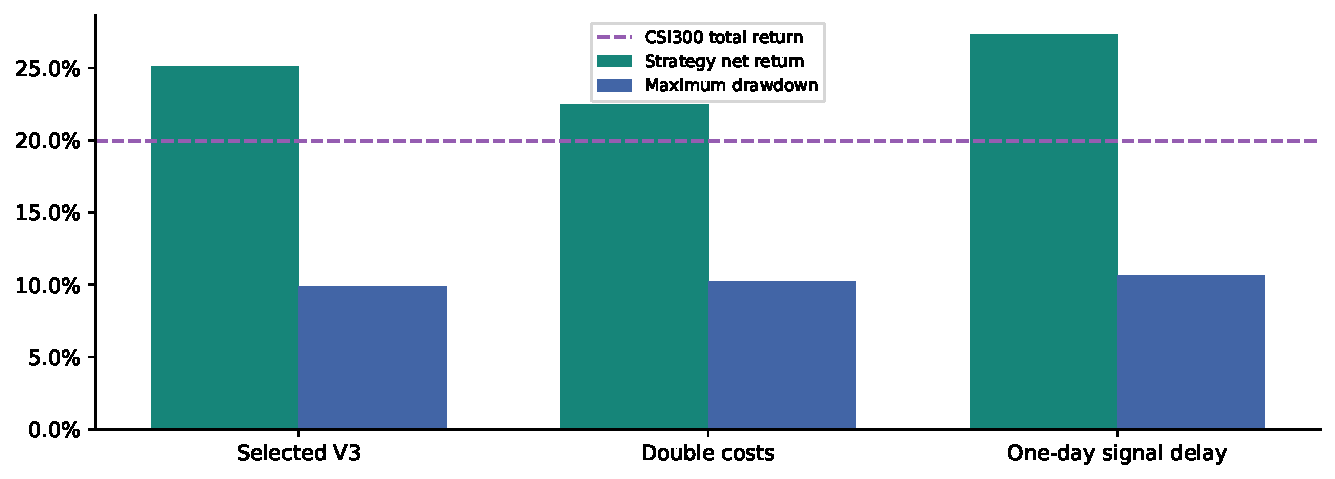
\includegraphics[width=.94\textwidth,height=.51\textheight,keepaspectratio]{figures/controls.pdf}\par
\scriptsize\begin{itemize}
\item 双倍费用：22.48\%；延后一日：27.31\%
\item 2023起连续收益44.09\%，最大回撤19.70\%
\end{itemize}
\note{双倍费用和延迟一天都重新运行完整账本，并超过同区间全收益指数。延迟一天更高不能据此改默认参数。另从2023起连续运行，避免每年重新起步；2024落后指数7.28个百分点，仍原样呈现。}
\end{frame}

\begin{frame}{因子诊断同时保留负结果}
\begin{block}{}878个形成日，逐日横截面IC与20日标签\end{block}
\centering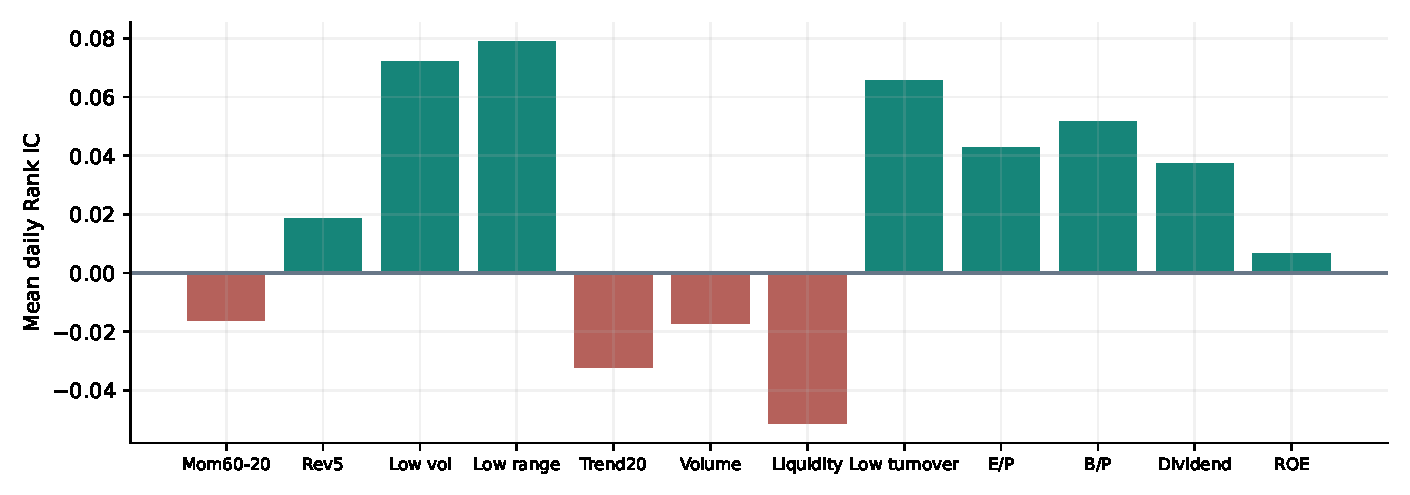
\includegraphics[width=.94\textwidth,height=.51\textheight,keepaspectratio]{figures/factor_ic.pdf}\par
\scriptsize\begin{itemize}
\item 低波动与低振幅较强，仍需检查信息冗余
\item 先形成五组，再匹配未来标签；不重新分组
\item 重叠20日收益均值不连乘成净值，不声称显著性
\end{itemize}
\note{这里展示中性化因子的平均Rank IC。低波动、低振幅和低换手较好，流动性和均线趋势为负。每一天先跨股票计算相关，再沿时间汇总；这与把全部股票日混在一起算一次相关不同。分组也先依据当日分数固定，再统计未来收益和缺失人数。因为标签重叠，相邻二十日收益并不独立，因此这些平均值属于诊断，不能直接称为可交易收益或显著alpha。}
\end{frame}

\begin{frame}{现场演示：版本、目标与账本}
\begin{block}{}两分钟切换最新、旧版与失败案例\end{block}
\small\begin{itemize}
\item 策略研究：查看价格/全收益指数和选择边界
\item 回测实验：默认最新V3，切换V2原预选
\item V1自由实验：查看明确的历史失败标记
\item 展开参数重跑：看版本、日期、费用及明细
\end{itemize}
\note{先打开策略研究说明25.13与两个指数。然后进入回测实验，确认默认滚动LightGBM；切换V2，收益应变为6.12并显示未超过指数；再切V1展示失败警示。最后返回V3，说明改参数会生成新的实验，旧结果不会混入。现场可用预热缓存演示。}
\end{frame}

\begin{frame}{平台满足研究与演示目标}
\begin{block}{}历史上跑赢指数；未来仍须前向验证\end{block}
\small\begin{itemize}
\item 达成：扣费后超过价格及全收益指数
\item 验证：52项测试、21个账本、独立复算
\item 保留：失败预选、8个候选、落后年份
\item 下一步：冻结V3，使用未来新数据检验
\end{itemize}
\note{最终交付包括可维护平台、完整策略版本、报告和演示。结果达到这段历史的目标，但不能保证未来赚钱或满分。最重要的研究边界是当前候选在看过最终历史结果后被选中，需要新的前向数据来验证。}
\end{frame}

\begin{frame}{备份：绩效与购买力口径}
\begin{block}{}期初净值参与第一日收益与最大回撤\end{block}
\[R_{real}=\frac{1+R_{strategy}}{1+\pi_{CPI}}-1\]
\small\begin{itemize}
\item 年化： (NAV末 / NAV初)\textasciicircum{}(252 / 交易日数) $-$ 1
\item Sharpe：$\sqrt{252}$ $\times$ 日超额均值 / 日超额样本标准差
\item CPI累计：逐月(1 + 月环比)相乘 $-$ 1
\item 实际收益：(1 + 策略收益) / (1 + CPI累计) $-$ 1
\end{itemize}
\note{回答口径问题时使用。无风险年利率默认零，日标准差ddof为一；零波动Sharpe记缺失。回撤高水位包含初始资金。CPI同比没有参与连乘。价差分组没有冒充可执行多空策略，费用加回也没有冒充无费用独立重跑。}
\end{frame}

\begin{frame}{备份：老师可能追问什么}
\begin{block}{}把选型、基准和失败讲清楚\end{block}
\small\begin{itemize}
\item 为什么不选最高收益？稳定树模型验证回撤超25\%
\item 为何不用CNN？因子列没有天然局部邻接
\item 是不是独立盲测？不是，明确披露事后选择
\item 来源：中证、Tushare、Qlib、sklearn、CogAlpha
\end{itemize}
\note{应如实回答：价值主题预选失败，滚动LightGBM是在本轮历史候选中进一步筛选的。价格和全收益指数分别给结论，ETF只是代理。我们保留52项测试、源码身份和独立复算，不能用工程验证来替代市场泛化证明。}
\end{frame}
\end{document}